\chapter{Experiments}\label{chp:experiments}

In this chapter we'll benchmark a WebRTC-based video conferencing solution for our test cases, to get a sense of how a peer-to-peer architecture performs.


\section{Test Setup}

To benchmark appear.in, our WebRTC-based video conferencing solution of choice, we have utilized a small cluster of desktop computers with web cameras, running the most recent versions of Mozilla Firefox\footnote{Version 36.0.4, latest version as of 2015.06.05 when the tests were run} and Google Chrome\footnote{Version 41.0.2272.101, latest version as of 2015.06.11 when the tests were run}. These two browsers was chosen since they collectively represent 85\% of the browser market (according to \cite{browser-stats}), and are powered by two different underlying engines. The goal of the benchmark is to get a sense of how the browsers -- and by extension, appear.in -- performs with regard to latency and bandwidth usage in our different test scenarios, and from that data observe how resources are shared among the nodes in a conversation.

Since the test covers two different browsers who do not share a common API (more on this later), measurements were done in two different ways. For Firefox, who do not expose timing data of WebRTC-streamms, a browser-external way of measuring end-to-end latencies was necessary. For this we synchronzed all the clocks in the cluster to the same \gls{NTP} server, and set another independent node -- also synced to the same time server -- to run a timer. Each of the nodes in the test filmed this timer, and with the same timer running locally in a terminal, the end-to-end latency could be extracted by taking regular screenshots, and finding the difference between the local timer and the timer as sent by the other nodes. See \autoref{fig:example-screenshot} for an example of how the screenshots looked.

\begin{figure}
    \centering
    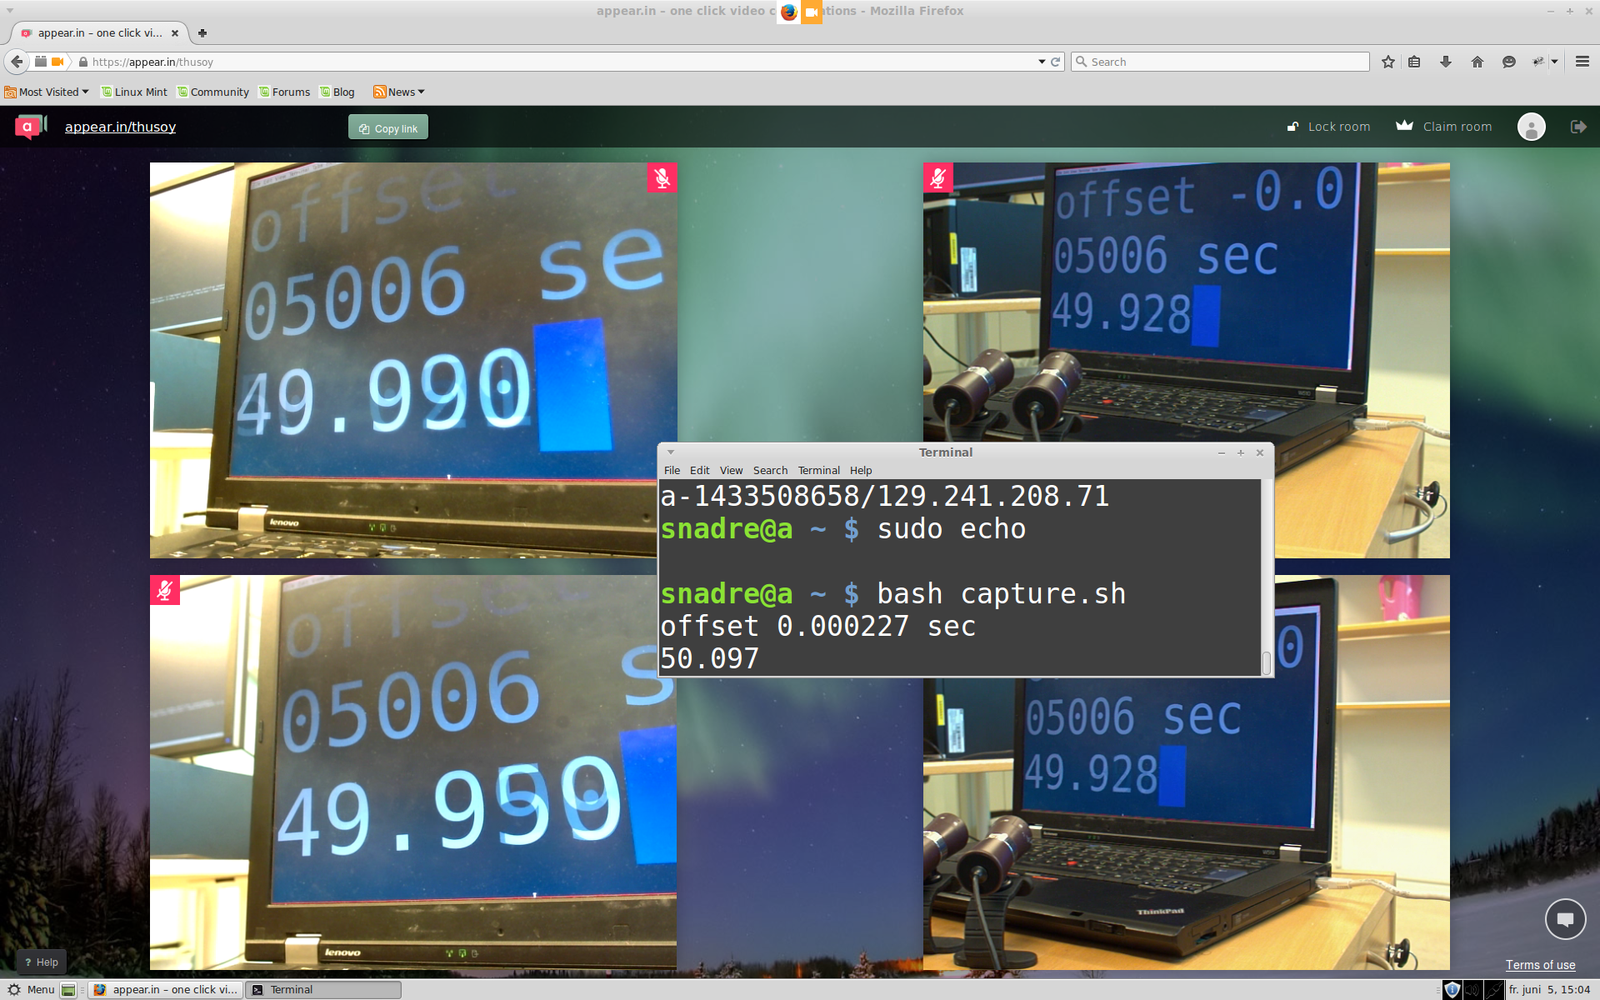
\includegraphics[width=.7\textwidth]{example-screenshot}
    \caption{An example screenshot from a test run on node A. The nodes are, from top left and clockwise, A, C, B and D. We can see from the difference between the local timestamp and A's own video stream that there's about 75ms of processing time in the browser before the image is sent (if we round A up to the almost visible 50.021 timestamp), and that the latencies from the other nodes are 31ms, 93ms and 93ms for B, C, and D, respectively.}
    \label{fig:example-screenshot}
\end{figure}

Bandwidth usage was measured by running \texttt{tcpdump} throughout the test run, and later extracting sent and received data with \texttt{tshark}.

For the Chrome tests, this was a bit simpler and less manual, as Chrome do provider timing data through the \texttt{getStats} API. Firefox also supports \texttt{getStats}, but does not return as much data as Chrome does, even though the data is assumed to be available internally in the browser.

\todo{Add note about order nodes enter conv.}

\todo{How to read graph chart}

\todo{How to read bandwidth}

\subsection{getStats}

The relevant values offered by the \texttt{getStats}-API on Chrome\footnote{Documentation is very lacking for the \texttt{getStats}-API, as the specification is not completed yet, so the most reliable reference is the source: \url{https://chromium.googlesource.com/external/webrtc/+/master/talk/app/webrtc/statstypes.cc}} is:

\subsubsection{Video Send}
\begin{itemize}
    \setlength\itemsep{.1em}
    \setlength\parsep{0pt}
    \setlength\parskip{0pt}
    \item bytesSent (\texttt{``106680''})
    \item googAvgEncodeMs (\texttt{``8''})
    \item googCaptureJitterMs (\texttt{``24''})
    \item googCaptureQueueDelayMsPerS (\texttt{``0''})
    \item googCodecName (\texttt{``VP8''})
    \item googBandwidthLimitedResolution (\texttt{``false''})
    \item googCpuLimitedResolution (\texttt{``false''})
    \item googViewLimitedResolution (\texttt{``false''})
    \item googRtt (\texttt{``81''})
    \item packetsLost (\texttt{``0''})
    \item packetsSent (\texttt{``131''})
\end{itemize}

\subsubsection{Video Receive}
\begin{itemize}
    \setlength\itemsep{.1em}
    \setlength\parsep{0pt}
    \setlength\parskip{0pt}
    \item bytesReceived (\texttt{``74557''})
    \item googCurrentDelayMs (\texttt{``25''})
    \item googDecodeMs (\texttt{``2''})
    \item googJitterBufferMs (\texttt{``11''})
    \item googMaxDecodeMs (\texttt{``4''})
    \item googMinPlayoutDelayMs (\texttt{``0''})
    \item googRenderDelayMs (\texttt{``10''})
    \item googTargetDelayMs (\texttt{``25''})
    \item packetsLost (\texttt{``0''})
    \item packetsReceived (\texttt{``109''})
\end{itemize}

To configure the cluster according to the different test cases, we utilized the Linux traffic control utility \texttt{tc}, which is capable of rate-limiting incoming and outgoing traffic, as well as delaying traffic destined for certain hosts. A small script was developed to act as a glue layer between a representation of a network and \texttt{tc}, making configuration repeatable and easily parametrized. The script is included in \autoref{chp:apply-case}.

Thus, applying a given test case is completely independent of the actual network utilized in the test cluster, keeping all intelligence on the nodes themselves. This removed the need for expensive routers or having to customize the application code, thus making the method application agnostic and applicable to any peer-to-peer solution, not just appear.in.

In contrast to most other video conferencing solutions, appear.in displays a node's own video stream just as big as the other streams in the conversation. This enables us to get a sense of how much time the browser spends processing the incoming video stream, as we can estimate this as the difference between the local timestamp and the timestamp of your own video stream as displayed in the browser. Since we're not benchmarking CPU usage in these tests, we can subtract this difference from the observed latencies between the other nodes, to only look at latencies originating in the network stack. Hence, all latencies reported in this thesis are lower than the actual observed end-to-end latencies by 50--70ms.

Ideally, testing would be automated and not require a running graphical environment, to allow it to be tested using remote servers. This could be possible using \texttt{node-webrtc}\footnote{\url{https://github.com/js-platform/node-webrtc}} or running a browser in a fake framebuffer like \texttt{Xvfb}\footnote{\url{http://www.x.org/releases/X11R7.6/doc/man/man1/Xvfb.1.xhtml}} and faking out a media stream\footnote{Chrome: \texttt{-{}-use-fake-device-for-media-stream}, Firefox: \texttt{getUserMedia(\{fake: true, <...>\})}. More info at \url{http://images.tmcnet.com/expo/webrtc-conference/presentations/san-jose-14/D3-2_Testing_v2_2.pdf}}. It is thus probably possible to automate this, but was considered out of scope for this thesis.

Firefox was chosen for these experiments due to its support for user stylesheets, which the Chrome team for some reason has abandoned support for in later versions. appear.in mirrors your own video stream when displayed back to yourself, probably since that's how most people are used to seeing themselves, but this is suboptimal when we want to retain some sanity while manually interpreting numbers shown this way. For browsers with support for user stylesheets, the fix is a simple matter of writing a stylesheet that flips your own image back\cprotect\footnote{For Firefox, this would mean putting the following in \texttt{~/.mozilla/firefox/<user-profile>/chrome/userContent.css}:
\begin{lstlisting}[language=CSS]
@-moz-document domain(appear.in) {
    div.local-client {
        transform: scaleX(-1);
    }
}
\end{lstlisting}}. When working with several machines, having the option to deploy changes like this to all machines with one single file without any other configuration changes is enormously gratifying.


\section{Caveats}

Our method is accurate in the sense that latencies observed are the actual end-to-end latencies that users would observe, but the precision of the timing values observed is not on the millisecond level we'd prefer. This is due to a number of factors, most notably the refresh rate of the screen running the timer and the framerate of the video, limiting the precision to $1s/60\approx17ms$ and $1s/30\approx33ms$ respectively. However, we can surpass this precision by averaging several samples taken during the test run, which is why we take several screenshots for each test case, once every 10s for at least a minute. The standard deviation of the measurements is reported in the graphs included later in this chapter, which should give some indication towards how accurate the average is.

Taking several samples to improve accuracy leads us to another weakness, which is the manual interpretation of the screenshots. Due to the frequency-related issues discussed above, many of the images include timestamps that are blurred, as the camera captured two underlying screen updates in the same frame, as shown in \autoref{fig:blurred-capture}.

\begin{figure}
    \centering
    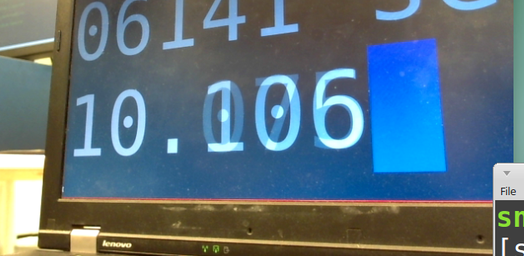
\includegraphics[width=.7\textwidth]{blurred-capture}
    \caption{A screenshot where a node has sent two overlaying timestamps. In this case interpreted as 10.106, which is reasonable as it's close to the expected 33ms increase from the previous 10.075.}
    \label{fig:blurred-capture}
\end{figure}

In general for these cases, the recorded timestamp was consistently interpreted to be the latest of what could be distinguished in the screenshot.

Even assuming that the timestamps are comprehensible and fairly accurate, there's still a possibility of human error when lots of numbers has to be recorded in this way. To minimize the risk of any mistyped numbers making it into the dataset, any number outside 1.5 standard deviations of the mean (a range which should include \todo{find actual range covered}80\% of the numbers observed) was verified once more. There's still a chance of smaller errors making it into the dataset, but we assume that these are small enough and distributed evenly among the nodes to not significantly influence any conclusions drawn.

As not enough cameras of any single model was available for the experiments, two different models\todo{Insert picture of the cameras here, or footnote} had to be used. These had slightly different performance characterstics; the cameras were put side by side with a timer and showed a mean difference of 39.6ms, but with a relatively large standard deviation of 19.5ms. As the same restrictions on screen refresh rates as discussed above, pretty much all the samples were at a 30ms or 60ms interval of each other.\footnote{Out of 20 samples, 1 was 0ms, 13 was 30ms, 5 was 60ms, and 1 was 90ms. Which really means in the range of that frame, that is in the range of 0--29ms difference, 30--60ms difference, and so on.} As the difference was assumed to be normally distributed, the mean was simply added to all measurements from the slower camera model to compensate.

For measuring bandwidth utilization between nodes, our method of using \texttt{tcpdump} is not entirely satisfactory, as there's no way to report actual \emph{consumed} bandwidth by the application. This is due to the traffic control features of the Linux kernel lying above where \texttt{libpcap}, the library that performs packet capture for \texttt{tcpdump}, listens in the network stack, meaning any incoming bandwidth reported will be before the rate limiting performed by \texttt{tc}. Thus, \texttt{tcpdump} cannot report the bandwidth actually consumed by application, only what was actually received by the network interface. Nonetheless, the bandwidth \emph{sent} by each node is what was actually sent by the application, but there's no guarantee that the node was actually capable of consuming it all. This is good enough for us though, as we can aggregate the data sent by all nodes to determine how saturated a given node's network link is.

While the method itself is application-agnostic, configuring nodes the way we do is not suitable for testing other architectures, such as the ones used by Hangouts and Skype. This is unfortunate, as a performance comparison between the different architectures would have been very interesting, but without running a local instance of the architecture under test, there's no way to achieve the internode latencies we desire. This follows from observing that if node A sends her video stream to a Google server, there's no way for her to signal to Google that when the stream is broadcast to nodes B and C, B's stream should be delayed by $x$ms, and the stream to C should be delayed $y$ms. It's also not possible for B and C to apply this latency on the receiving side, as they'd have to split the incoming stream for Google into separate streams for each of the transmitting nodes, which would require both getting access to the DTLS keys used by the web browser to encrypt the traffic, and being capable of splitting the stream and rejoining it again without interfering with the browser.


\section{Method}\label{sec:method}

(screensharing scrapped due to framerate artifically limited too severly, did not run any custom code since the solution needed to be (relatively) service agnostic, and could not modify code since it would need to be tagged in the video stream somehow. Some for appear.in, would need to be included in the sdp stream, and extracted -> way too much work).


\section{Results}

To get a sense of how appear.in performs under optimal conditions, a test run was performed with 3, 4 and 7 nodes in a conversation, without any traffic shaping. We would expect both bandwidth and latencies to be fairly even among all the nodes, as the only thing different between them is the time they entered the conversation. Since they were given some time to stabilize before the measurements was started, some fairness should have been achieved.

As we see in \autoref{fig:vanilla-3p}, bitrates between the nodes are identical, as expected. From the latency measurements there seems to be a slight inclination towards the latest arriving node having somewhat higher latencies outgoing, but the difference is negligible in practice.

\subsection{Mozilla Firefox}

\begin{figure}
    \centering
    \begin{subfigure}[t]{.48\textwidth}
        \centering
        \begin{tikzpicture}
        \begin{axis}[
            ybar,
            ylabel=Bitrate (bps),
            xtick=data,
            width=\textwidth,
            symbolic x coords={A,B,C},
            enlargelimits=0.15
            ]
            \input{data/appear.in-vanilla-3p/bitrate.tex}
        \end{axis}
        \end{tikzpicture}
        \subcaption{Outgoing traffic from each node}
    \end{subfigure}
    \hfill
    \begin{subfigure}[t]{.48\textwidth}
        \centering
        \begin{tikzpicture}
        \begin{axis}[
            ybar,
            compat=newest,
            ylabel=Latency (ms),
            xtick=data,
            width=\textwidth,
            symbolic x coords={A,B,C},
            enlargelimits=0.15,
            nodes near coords=\raisebox{.3cm}{\pgfmathprintnumber{\pgfplotspointmeta}}
            ]
            \input{data/appear.in-vanilla-3p/latency.tex}
        \end{axis}
        \end{tikzpicture}
        \subcaption{Outgoing latencies for each node}
    \end{subfigure}
    \caption{Test results for three nodes without traffic shaping}
    \label{fig:vanilla-3p}
\end{figure}

Adding another node to the mix, we get the results as shown in \autoref{fig:vanilla-4p}. We see that the bandwidth between the nodes is the same 2.1Mpbs that we saw when there was only three nodes in the conversation, which we can assume is the default transmit bitrate for appear.in. We can also see the same phenomena as in the three node case, that the later arrivals tend to have a slightly higher latency to the nodes first to arrive in the conversation. However, the later nodes (C and D) does not display this phenomena between themselves, thus since all the observations are within one standard deviation of each other we'll not spend any more time investigating this.


\begin{figure}
    \centering
    \begin{subfigure}[t]{.9\textwidth}
        \centering
        \begin{tikzpicture}
        \begin{axis}[
            ybar,
            ylabel=Bitrate (bps),
            xtick=data,
            width=\textwidth,
            bar width=10,
            height=240,
            symbolic x coords={A,B,C,D},
            enlargelimits=0.15
            ]
            \input{data/appear.in-vanilla-4p/bitrate.tex}
        \end{axis}
        \end{tikzpicture}
        \subcaption{Outgoing traffic from each node}
    \end{subfigure}
    \begin{subfigure}[t]{.9\textwidth}
        \centering
        \begin{tikzpicture}
        \begin{axis}[
            ybar,
            compat=newest,
            ylabel=Latency (ms),
            xtick=data,
            width=\textwidth,
            symbolic x coords={A,B,C,D},
            bar width=10,
            height=240,
            enlargelimits=0.15,
            nodes near coords=\raisebox{.3cm}{\pgfmathprintnumber{\pgfplotspointmeta}}
            ]
            \input{data/appear.in-vanilla-4p/latency.tex}
        \end{axis}
        \end{tikzpicture}
        \subcaption{Outgoing latencies for each node}
    \end{subfigure}
    \caption{Test results for four nodes without traffic shaping}
    \label{fig:vanilla-4p}
\end{figure}

In the final test without traffic shaping, we step it up to seven nodes in the conversation. The results can be seen in \autoref{fig:vanilla-7p}, and largely mirror what we saw in the smaller experiements. Latencies are a bit higher, which can probably be expected due to the increase in traffic, and apart from a bandwidth deviation on node E, all nodes continue transmitting on the previously observed 2.1Mbps. Why node E's behavior is worse than the other nodes are unknown, but it could be related to node E being on a busier subnet than the other nodes (E was the only node in the test cluster on its subnet).


\begin{figure}
    \centering
    \begin{subfigure}[t]{\textwidth}
        \centering
        \begin{tikzpicture}
        \begin{axis}[
            ybar,
            ylabel=Bitrate (bps),
            xtick=data,
            width=\textwidth,
            bar width=3,
            height=240,
            symbolic x coords={A,B,C,D,E,F,G},
            enlargelimits=0.10
            ]
            \input{data/appear.in-vanilla-7p/bitrate.tex}
        \end{axis}
        \end{tikzpicture}
        \subcaption{Outgoing traffic from each node}
    \end{subfigure}
    \begin{subfigure}[t]{\textwidth}
        \centering
        \begin{tikzpicture}
        \begin{axis}[
            ybar,
            compat=newest,
            ylabel=Latency (ms),
            xtick=data,
            width=\textwidth,
            symbolic x coords={A,B,C,D,E,F,G},
            bar width=3,
            height=240,
            enlargelimits=0.10,
            major grid style=dashed,
            ymajorgrids
            ]
        \input{data/appear.in-vanilla-7p/latency.tex}
        \end{axis}
        \end{tikzpicture}
        \subcaption{Outgoing latencies for each node}
    \end{subfigure}
    \caption{Test results for seven nodes without traffic shaping}
    \label{fig:vanilla-7p}
\end{figure}


\todo[inline]{[minor] If time, define custom color set for graphing, based possibly either on solarized or http://clrs.cc/}


For our first test case, ``Asia'', the results are shown in \autoref{fig:asia-bitrate}. We can tell that even though node B transmits 0.5Mbps to each of the other nodes, neither of them receive recent data frequent enough to keep an acceptable conversation with node B. The good thing is that even though node B suffers greatly in this case, the flow between A and C is unaffected.

\begin{figure}
    \centering
    \begin{subfigure}[t]{.48\textwidth}
        \centering
        \begin{tikzpicture}
        \begin{axis}[
            ybar,
            ylabel=Bitrate (bps),
            xtick=data,
            width=\textwidth,
            bar width=8,
            symbolic x coords={A,B,C},
            enlargelimits=0.15,
            ]
            \input{data/appear.in-asia/bitrate.tex}
        \end{axis}
        \end{tikzpicture}
        \subcaption{Outgoing traffic from each node}
    \end{subfigure}
    \hfill
    \begin{subfigure}[t]{.48\textwidth}
        \centering
        \begin{tikzpicture}
        \begin{axis}[
            ybar,
            compat=newest,
            ylabel=Latency (ms),
            xtick=data,
            ymax=1000,
            width=\textwidth,
            bar width=8,
            symbolic x coords={A,B,C},
            enlargelimits=0.15,
            nodes near coords=\raisebox{.3cm}{\pgfmathprintnumber{\pgfplotspointmeta}}
            ]
            \input{data/appear.in-asia/latency.tex}
        \end{axis}
        \end{tikzpicture}
        \subcaption{Outgoing latencies for each node}
    \end{subfigure}
    \caption{Test results for the ``asia'' test case. The out-of-bounds latencies are are all larger than 24s.}
    \label{fig:asia-bitrate}
\end{figure}

Next up we have the ``standup'' test case, as seen in \autoref{fig:standup}. The key challenge in this case node D, with only 6Mbps available on the downlink, slightly upped by node C with 8Mbps. Node C doesn't have any troubles in this test, but node D is completely satured, receiving 2.1Mbps from each of the other three nodes. Even though node D sends to its fullest capacity, hardly anything of this is correctly received by the other nodes, as can be seen from the latencies incurred. This probably implies that among the data Firefox is actually putting onto the wire, not enough of it reaches the destinations unfragmented, and thus the receiver is incapable of recontructing a complete frame to show to the user.

\begin{figure}
    \centering
    \begin{subfigure}[t]{.9\textwidth}
        \centering
        \begin{tikzpicture}
        \begin{axis}[
            ybar,
            ylabel=Bitrate (bps),
            xtick=data,
            width=\textwidth,
            bar width=8,
            height=240,
            symbolic x coords={A,B,C,D},
            enlargelimits=0.15
            ]
            \input{data/appear.in-standup/bitrate.tex}
        \end{axis}
        \end{tikzpicture}
        \subcaption{Outgoing traffic from each node}
    \end{subfigure}
    \begin{subfigure}[t]{.9\textwidth}
        \centering
        \begin{tikzpicture}
        \begin{axis}[
            ybar,
            ylabel=Latency (ms),
            xtick=data,
            width=\textwidth,
            ymax=1000,
            bar width=8,
            height=240,
            symbolic x coords={A,B,C,D},
            enlargelimits=0.15,
            nodes near coords=\raisebox{.3cm}{\pgfmathprintnumber{\pgfplotspointmeta}}
            ]
            \input{data/appear.in-standup/latency.tex}
        \end{axis}
        \end{tikzpicture}
        \subcaption{Outgoing latencies for each node}
    \end{subfigure}
    \caption{Test results for the ``standup'' test case.}
    \label{fig:standup}
\end{figure}


\begin{figure}
    \centering
    \begin{subfigure}[t]{\textwidth}
        \centering
        \begin{tikzpicture}
        \begin{axis}[
            ybar,
            ylabel=Bitrate (bps),
            xtick=data,
            width=\textwidth,
            bar width=3,
            height=240,
            symbolic x coords={A,B,C,D,E,F,G},
            enlargelimits=0.10
            ]
            \input{data/appear.in-friends/bitrate.tex}
        \end{axis}
        \end{tikzpicture}
        \subcaption{Outgoing traffic from each node}
    \end{subfigure}
    \begin{subfigure}[t]{\textwidth}
        \centering
        \begin{tikzpicture}
        \begin{axis}[
            ybar,
            ymode=log,
            axis x line=bottom,
            ylabel=Latency (ms),
            xtick=data,
            width=\textwidth,
            symbolic x coords={A,B,C,D,E,F,G},
            bar width=3,
            height=240,
            enlargelimits=0.10,
            major grid style=dashed,
            ymajorgrids
            ]
            \input{data/appear.in-friends/latency.tex}
        \end{axis}
        \end{tikzpicture}
        \subcaption{Outgoing latencies for each node}
    \end{subfigure}
    \caption{Test results for the ``friends'' test case, log scale}
    \label{fig:friends-log}
\end{figure}

\todo{Decide whether to group cases together, or bitrates/latencies with/without traffic shaping}

Last out is the ``friends'' test case. As there's a lot of data points for this case, the results have been split in two; one logarithmic view giving a rough overview of how the nodes performed (\autoref{fig:friends-log}), and one cropped view, where only edges with latency less than 500ms is included (\autoref{fig:friends-lin}). As we can see from the linear chart, there's only four nodes that observe latencies below 500ms, and not even all of those can reasonably be expected to be able to hold a conversation. A and B can talk together; A and E can talk, although a little more strained with latencies around 400ms. B and E can not talk, as B doesn't receive E's stream in reasonable time; B and F however \emph{can} talk together.

To summarize, out of 42 pairs of nodes in the test case, only three of them is able to communicate bidirectionally. In practice, this is a conversation all parties abandon immediately, as it's useless.

\begin{figure}
    \centering
    \begin{tikzpicture}
    \begin{axis}[
        ybar,
        ylabel=Latency (ms),
        xtick=data,
        width=\textwidth,
        symbolic x coords={A,B,C,D,E,F,G},
        bar width=3,
        height=240,
        enlargelimits=0.15,
        major grid style=dashed,
        ymajorgrids
        ]
        %% Traffic going out to A
\addplot+[error bars/.cd,y dir=both, y explicit]
coordinates{
    (A,0) +- (0.0, 0)
    (B,140) +- (0.0, 16)
    (C,0) +- (0.0, 0)
    (D,0) +- (0.0, 0)
    (E,410) +- (0.0, 87)
    (F,0) +- (0.0, 0)
    (G,0) +- (0.0, 0)
    };

%% Traffic going out to B
\addplot+[error bars/.cd,y dir=both, y explicit]
coordinates{
    (A,153) +- (0.0, 6)
    (B,0) +- (0.0, 0)
    (C,0) +- (0.0, 0)
    (D,0) +- (0.0, 0)
    (E,457) +- (0.0, 147)
    (F,356) +- (0.0, 86)
    (G,0) +- (0.0, 0)
    };

%% Traffic going out to C
\addplot+[error bars/.cd,y dir=both, y explicit]
coordinates{
    (A,156) +- (0.0, 14)
    (B,141) +- (0.0, 20)
    (C,0) +- (0.0, 0)
    (D,0) +- (0.0, 0)
    (E,0) +- (0.0, 0)
    (F,0) +- (0.0, 0)
    (G,0) +- (0.0, 0)
    };

%% Traffic going out to D
\addplot+[error bars/.cd,y dir=both, y explicit]
coordinates{
    (A,0) +- (0.0, 0)
    (B,0) +- (0.0, 0)
    (C,0) +- (0.0, 0)
    (D,0) +- (0.0, 0)
    (E,300) +- (0.0, 58)
    (F,143) +- (0.0, 12)
    (G,0) +- (0.0, 0)
    };

%% Traffic going out to E
\addplot+[error bars/.cd,y dir=both, y explicit]
coordinates{
    (A,429) +- (0.0, 41)
    (B,0) +- (0.0, 0)
    (C,0) +- (0.0, 0)
    (D,0) +- (0.0, 0)
    (E,0) +- (0.0, 0)
    (F,0) +- (0.0, 0)
    (G,0) +- (0.0, 0)
    };

%% Traffic going out to F
\addplot+[error bars/.cd,y dir=both, y explicit]
coordinates{
    (A,363) +- (0.0, 21)
    (B,373) +- (0.0, 19)
    (C,0) +- (0.0, 0)
    (D,0) +- (0.0, 0)
    (E,225) +- (0.0, 35)
    (F,0) +- (0.0, 0)
    (G,0) +- (0.0, 0)
    };

%% Traffic going out to G
\addplot+[error bars/.cd,y dir=both, y explicit]
coordinates{
    (A,0) +- (0.0, 0)
    (B,0) +- (0.0, 0)
    (C,0) +- (0.0, 0)
    (D,0) +- (0.0, 0)
    (E,0) +- (0.0, 0)
    (F,0) +- (0.0, 0)
    (G,0) +- (0.0, 0)
    };

\legend{A, B, C, D, E, F, G}

    \end{axis}
    \end{tikzpicture}
    \caption{Observed latencies in the ``friends'' test case, results below 500ms only, linear scale}
    \label{fig:friends-lin}
\end{figure}

\todo[inline]{Add example chart with guide for how to read values. What's depicted over A is the latency from those nodes TO A.}

\subsection{Google Chrome}

Now to the Chrome tests.

\begin{figure}
    \centering
    \begin{subfigure}[t]{.48\textwidth}
        \centering
        \begin{tikzpicture}
        \begin{axis}[
            ybar,
            ylabel=Latency (ms),
            xtick=data,
            width=\textwidth,
            bar width=8,
            height=240,
            ymax=150,
            symbolic x coords={A,B,C,D},
            enlargelimits=0.15
            ]
            \input{data/appear.in-capture-vanilla-3p/latency-timer.tex}
        \end{axis}
        \end{tikzpicture}
        \subcaption{Latencies measured by filming a timer}
    \end{subfigure}
    \hfill
    \begin{subfigure}[t]{.48\textwidth}
        \centering
        \begin{tikzpicture}
        \begin{axis}[
            ybar,
            ylabel=Latency (ms),
            xtick=data,
            width=\textwidth,
            ymax=150,
            bar width=8,
            height=240,
            symbolic x coords={A,B,C,D},
            enlargelimits=0.15,
            ]
            \input{data/appear.in-capture-vanilla-3p/latency-getstats.tex}
        \end{axis}
        \end{tikzpicture}
        \subcaption{Latencies reported by \texttt{getStats}}
    \end{subfigure}
    \caption{Timer broadcasting and getStats compared for three nodes without traffic shaping. Note that the timer broadcasting has only 6 samples, while \texttt{getStats} has 80.}
    \label{fig:standup}
\end{figure}

\begin{figure}
    \centering
    \begin{subfigure}[t]{.48\textwidth}
        \centering
        \begin{tikzpicture}
        \begin{axis}[
            ybar,
            ylabel=Latency (ms),
            xtick=data,
            width=\textwidth,
            bar width=8,
            height=240,
            ymax=300,
            symbolic x coords={A,B,C,D},
            enlargelimits=0.15
            ]
            \input{data/appear.in-capture-asia/latency-timer.tex}
        \end{axis}
        \end{tikzpicture}
        \subcaption{Latencies measured by filming a timer}
    \end{subfigure}
    \hfill
    \begin{subfigure}[t]{.48\textwidth}
        \centering
        \begin{tikzpicture}
        \begin{axis}[
            ybar,
            ylabel=Latency (ms),
            xtick=data,
            width=\textwidth,
            ymax=300,
            bar width=8,
            height=240,
            symbolic x coords={A,B,C,D},
            enlargelimits=0.15,
            ]
            \input{data/appear.in-capture-asia/latency-getstats.tex}
        \end{axis}
        \end{tikzpicture}
        \subcaption{Latencies reported by \texttt{getStats}}
    \end{subfigure}
    \caption{Timer broadcasting and getStats compared for the asia test case. Note that the timer broadcasting has only 6 samples, while \texttt{getStats} has 80.}
    \label{fig:standup}
\end{figure}


\begin{figure}
    \centering
    \begin{subfigure}[t]{\textwidth}
        \centering
        \begin{tikzpicture}
        \begin{axis}[
            ybar,
            ymax=950,
            ylabel=Latency (ms),
            xtick=data,
            width=\textwidth,
            symbolic x coords={A,B,C,D,E,F,G},
            bar width=3,
            height=240,
            enlargelimits=0.10,
            major grid style=dashed,
            ymajorgrids
            ]
            \input{data/appear.in-capture-vanilla-7p/latency-getstats.tex}
        \end{axis}
        \end{tikzpicture}
        \subcaption{Latencies measured without traffic shaping, seven nodes}
    \end{subfigure}
    \begin{subfigure}[t]{\textwidth}
        \centering
        \begin{tikzpicture}
        \begin{axis}[
            ybar,
            ymax=950,
            ylabel=Latency (ms),
            xtick=data,
            width=\textwidth,
            symbolic x coords={A,B,C,D,E,F,G},
            bar width=3,
            height=240,
            enlargelimits=0.10,
            major grid style=dashed,
            ymajorgrids
            ]
            \input{data/appear.in-capture-friends/latency-getstats.tex}
        \end{axis}
        \end{tikzpicture}
        \subcaption{Latencies observed with traffic shaping, ``friends'' test case}
    \end{subfigure}
    \caption{Observed latencies in a conversation with seven nodes, with and without traffic shaping}
    \label{fig:vanilla-7p-getstats}
\end{figure}

\begin{figure}
    \centering
    \begin{subfigure}[t]{\textwidth}
        \centering
        \begin{tikzpicture}
        \begin{axis}[
            ybar,
            ymax=950,
            ylabel=Latency (ms),
            xtick=data,
            width=\textwidth,
            symbolic x coords={A,B,C,D,E,F,G},
            bar width=3,
            height=240,
            enlargelimits=0.10,
            major grid style=dashed,
            ymajorgrids
            ]
            \input{data/appear.in-final-vanilla-7p/latency-getstats.tex}
        \end{axis}
        \end{tikzpicture}
        \subcaption{Latencies measured without traffic shaping, seven nodes}
    \end{subfigure}
    \begin{subfigure}[t]{\textwidth}
        \centering
        \begin{tikzpicture}
        \begin{axis}[
            ybar,
            ymax=950,
            ylabel=Latency (ms),
            xtick=data,
            width=\textwidth,
            symbolic x coords={A,B,C,D,E,F,G},
            bar width=3,
            height=240,
            enlargelimits=0.10,
            major grid style=dashed,
            ymajorgrids
            ]
            \input{data/appear.in-final-friends/latency-getstats.tex}
        \end{axis}
        \end{tikzpicture}
        \subcaption{Latencies observed with traffic shaping, ``friends'' test case}
    \end{subfigure}
    \caption{Observed latencies in a conversation with seven nodes, with and without traffic shaping FINAL DATA}
    \label{fig:vanilla-7p-getstats}
\end{figure}


\begin{figure}
    \centering
    \begin{subfigure}[t]{\textwidth}
        \centering
        \begin{tikzpicture}
        \begin{axis}[
            ybar,
            ymax=950,
            ylabel=Latency (ms),
            xtick=data,
            width=\textwidth,
            symbolic x coords={A,B,C,D},
            bar width=8,
            height=240,
            enlargelimits=0.15,
            major grid style=dashed,
            ymajorgrids
            ]
            \input{data/appear.in-capture-vanilla-4p/latency-getstats.tex}
        \end{axis}
        \end{tikzpicture}
        \subcaption{Latencies measured without traffic shaping, seven nodes}
    \end{subfigure}
    \begin{subfigure}[t]{\textwidth}
        \centering
        \begin{tikzpicture}
        \begin{axis}[
            ybar,
            ymax=950,
            ylabel=Latency (ms),
            xtick=data,
            width=\textwidth,
            symbolic x coords={A,B,C,D},
            bar width=8,
            height=240,
            enlargelimits=0.15,
            major grid style=dashed,
            ymajorgrids
            ]
            \input{data/appear.in-final-standup/latency-getstats.tex}
        \end{axis}
        \end{tikzpicture}
        \subcaption{Latencies observed with traffic shaping, ``standup'' test case}
    \end{subfigure}
    \caption{Observed latencies in a conversation with seven nodes, with and without traffic shaping}
    \label{fig:vanilla-7p-getstats}
\end{figure}

\begin{figure}
    \centering
    \begin{subfigure}[t]{\textwidth}
        \centering
        \begin{tikzpicture}
        \begin{axis}[
            ybar,
            ylabel=Bitrate (bps),
            xtick=data,
            width=\textwidth,
            symbolic x coords={A,B,C,D,E,F,G},
            bar width=8,
            height=240,
            enlargelimits=0.15,
            major grid style=dashed,
            ymajorgrids
            ]
            \input{data/appear.in-capture-vanilla-4p/bitrate-getstats.tex}
        \end{axis}
        \end{tikzpicture}
        \subcaption{Observed bitrates without traffic shaping, seven nodes}
    \end{subfigure}
    \begin{subfigure}[t]{\textwidth}
        \centering
        \begin{tikzpicture}
        \begin{axis}[
            ybar,
            ylabel=Bitrate (bps),
            xtick=data,
            width=\textwidth,
            symbolic x coords={A,B,C,D,E,F,G},
            bar width=8,
            height=240,
            enlargelimits=0.15,
            major grid style=dashed,
            ymajorgrids
            ]
            \input{data/appear.in-capture-standup/bitrate-getstats.tex}
        \end{axis}
        \end{tikzpicture}
        \subcaption{Latencies observed with traffic shaping, ``standup'' test case}
    \end{subfigure}
    \caption{Observed bitrates in a conversation with seven nodes, with and without traffic shaping}
    \label{fig:vanilla-7p-getstats}
\end{figure}


\begin{figure}
    \centering
    \begin{subfigure}[t]{\textwidth}
        \centering
        \begin{tikzpicture}
        \begin{axis}[
            ybar,
            ylabel=Bitrate (bps),
            xtick=data,
            width=\textwidth,
            symbolic x coords={A,B,C,D,E,F,G},
            bar width=3,
            height=240,
            enlargelimits=0.15,
            major grid style=dashed,
            ymajorgrids
            ]
            \input{data/appear.in-capture-vanilla-7p/bitrate-getstats.tex}
        \end{axis}
        \end{tikzpicture}
        \subcaption{Latencies measured without traffic shaping, seven nodes}
    \end{subfigure}
    \begin{subfigure}[t]{\textwidth}
        \centering
        \begin{tikzpicture}
        \begin{axis}[
            ybar,
            ylabel=Bitrate (bps),
            xtick=data,
            width=\textwidth,
            symbolic x coords={A,B,C,D,E,F,G},
            bar width=3,
            height=240,
            enlargelimits=0.15,
            major grid style=dashed,
            ymajorgrids
            ]
            \input{data/appear.in-capture-friends/bitrate-getstats.tex}
        \end{axis}
        \end{tikzpicture}
        \subcaption{bitrates observed with traffic shaping, ``friends'' test case}
    \end{subfigure}
    \caption{Observed bitrates in a conversation with seven nodes, with and without traffic shaping}
    \label{fig:friends-getstats-bitrates}
\end{figure}

\autoref{fig:friends-getstats-bitrates} shows that for resource-constrained nodes, those resources are not distributed evenly among its peers. We see this in the data for node G, which is constrained to 9/4 bandwidth. Of it's 4Mbps, we see that node E receives a little more than 1Mbps of this, while the two other nearby nodes (D and F) lie around 500kbps each. Among the remote nodes, node C receives $\approx$350kbps, while A and B share the scraps that remain, with $\approx$200kbps each.

We observe something similar for nodes C and D, which are constrained to 8Mbps and 9Mbps, respectively. Well, almost -- node C is well received by nodes B, D and E, while nodes A and F are left with hardly anything -- which shows that being local or remote \emph{does not} seem to significantly influence who gets a fair share. Granted, this dataset is only from one single test run, more data is needed to say anything conclusively about whether this is expected behavior, but our data seem to imply that even a minute is not enough to reach fairness for Chrome/libjingle.

Node D repeats much of what we saw in node C, but with a stronger bias towards \emph{remote} nodes, which all got more than any individual local node. This might be due to D being the first of the second group into the conversation, establishing connections with the remote nodes before any of the other local nodes are present. Thus when the other nodes in D's group joins, they get to share whatever capacity D has left. How the distribution evolves with time was not studied in this thesis, but might provide insight into how long it would take to reach fairness.

In any case, if it takes more than 10-30 seconds to establish fairness, we consider it likely that the users will leave the platform and not wait for stuff to smoothen out, at least if video is of any importance in the conversation. Audio will not be hit as hard by uneven distribution, but if you're goal as a service provider is to deliver video conferencing, video quality and quick connection times will be how you're compared to other providers.

Uneven uplink distribution is not only bad for fairness in the conversation, but also for battery consumption. We can assume node G's video is encoded at least three times, possibly four in this test case\footnote{A and B might be receiving the same stream, C and D too (and possibly F as well), and E has a stream of its own}, even though all of the nodes have spare downlink capacity for sharing one $\approx$600kbps stream ($4\text{Mbit}/6$).
